\documentclass{article}
 
\usepackage[spanish]{babel}
\usepackage{listings}
\usepackage{epsfig} 
\usepackage{float}
 \usepackage{hyperref}
 \usepackage{color}
\usepackage{graphicx} % figuras
\usepackage{subfigure} % subfiguras
\usepackage[dvipsnames]{xcolor}
\usepackage{fancyvrb}
%\usepackage{multicol}
%\usepackage{url}
%\renewcommand{\UrlFont}{\small}
\setlength{\parskip}{0.25 cm}
\setlength{\parindent}{0pt}

%%%----------------------------------------------                 Datos              -----------------------------------------------------------
\title{Complejidad asintótica}
\author{4166}
%\institute{PISIS UANL}
%\email{hhector.garcialpz@uanl.edu.mx}
\date{\today}

\begin{document}
\maketitle
%%%--------------------------------------------                 Introduccion              -----------------------------------------------------
\section*{Introducción}
Distintos algoritmos se pueden usar para resolver los mismos problemas; el desempeño de los algoritmos es la manera de evaluar a los mismos en base a su eficiencia en la resolución de dichos problemas. Existen distintos métodos para evaluar del desempeño, esto se debe al tipo de algoritmos y sus problemas. En este documento se verá que afecta directamente el desempeño de ciertos algoritmos de \texttt{Networkx}.

\definecolor{mygreen}{rgb}{0,0.6,0}
\definecolor{mygray}{rgb}{0.5,0.5,0.5}
\definecolor{mymauve}{rgb}{0.58,0,0.82}
\lstset{ 
  backgroundcolor=\color{white},   % choose the background color; you must add \usepackage{color} or \usepackage{xcolor}; should come as last argument
  basicstyle=\footnotesize,        % the size of the fonts that are used for the code
  breakatwhitespace=false,         % sets if automatic breaks should only happen at whitespace
  breaklines=true,                 % sets automatic line breaking
  captionpos=b,                    % sets the caption-position to bottom
  commentstyle=\color{mygreen},    % comment style
  deletekeywords={...},            % if you want to delete keywords from the given language
  escapeinside={\%*}{*)},          % if you want to add LaTeX within your code
  extendedchars=true,              % lets you use non-ASCII characters; for 8-bits encodings only, does not work with UTF-8
  firstnumber=1,                % start line enumeration with line 1000
  frame=single,	                   % adds a frame around the code
  keepspaces=true,                 % keeps spaces in text, useful for keeping indentation of code (possibly needs columns=flexible)
  keywordstyle=\color{blue},       % keyword style
  language=Octave,                 % the language of the code
  morekeywords={*,...},            % if you want to add more keywords to the set
  numbers=left,                    % where to put the line-numbers; possible values are (none, left, right)
  numbersep=5pt,                   % how far the line-numbers are from the code
  numberstyle=\tiny\color{mygray}, % the style that is used for the line-numbers
  rulecolor=\color{black},         % if not set, the frame-color may be changed on line-breaks within not-black text (e.g. comments (green here))
  showspaces=false,                % show spaces everywhere adding particular underscores; it overrides 'showstringspaces'
  showstringspaces=false,          % underline spaces within strings only
  showtabs=false,                  % show tabs within strings adding particular underscores
  stepnumber=1,                    % the step between two line-numbers. If it's 1, each line will be numbered
  stringstyle=\color{mymauve},     % string literal style
  tabsize=2,	                   % sets default tabsize to 2 spaces
  title=\lstname                   % show the filename of files included with \lstinputlisting; also try caption instead of title
}

\section{Especificaciones técnicas}
La computadora en la que se corrió los algoritmos es una Macbook Pro, cuyo procesador es un Intel Core i5 de 2.3 GHz. Tiene una memoria RAM de 8 GB 2133 MHz.
%%%--------------------------------------------                 Algoritmos              -----------------------------------------------------
\section{Algoritmos}
Los algoritmos a implementar son los siguientes.
\subsection*{\texttt{maximum\_flow\_value()}}
Este algoritmo recibe como entrada un un grafo no orientado con capacidad en sus aristas junto con un par de nodos, el nodo \textit{fuente} que es de donde parte el flujo y el nodo \textit{sumidero} que es a donde llega el flujo. Devuelve el valor del flujo máximo soportado entre los nodos fuente y sumidero.

Utiliza el método de la etiqueta mas alta, es decir, de tomar el camino por el cual hay mas capacidad de aumento de flujo.

\subsection*{\texttt{flow.edmonds\_karp()}}
Este algoritmo recibe como entrada un grafo con capacidad junto con los nodos fuente y sumidero; lo que devuelve es la \textit{red residual} después de haber calculado el flujo máximo.

Tiene rasgos parecidos al algoritmo de Ford-Fulkerson pero la diferencia más significativa es que el algoritmo de Edmonds Karp busca el camino mas corto para encontrar una ruta de aumento, es decir, explora todos los caminos posibles entre la fuente y el sumidero buscando cuales tienen capacidad disponible. 

\subsection*{\texttt{flow.boykov\_kolmogorov()}}
Este algoritmo devuelve la red residual resultante después de calcular el flujo máximo, utilizando el algoritmo  Boykov-Kolmogorov.
%%%--------------------------------------------                 Generadores             -----------------------------------------------------
\section{Generadores}
Los generadores de grafos implementados fueron los siguientes.

\subsection*{\texttt{dense\_gnm\_random\_graph()}}
Este generador de grafos toma como parámetros la cantidad de nodos y aristas que se desean obtener; y devuele un grafo de entre los posibles grafos que cumplen con esos parámetros.

\subsection*{\texttt{random\_graphs.barabasi\_albert\_graph()}}
Este comando genera grafos aleatorios agregando las aristas de manera preferencial. Al generador se le dan los parámetros \textit{n} y \textit{m} que representan los nodos totales y el número de aristas a unir desde un nuevo nodo a los nodos existentes de acuerdo al algoritmo de Barabási-Albert.

\subsection*{\texttt{duplication.duplication\_divergence\_graph()}}
A este generador se le dan los parámetros \textit{n} y \textit{p} que representan el total de nodos y la probabilidad de retención de aristas incidentes a los nodos originales.

%%%--------------------------------------------                 Metodología              -----------------------------------------------------
\section{Metodología}
El interés de este estudio es ver que variables influyen en el tiempo del algoritmo y de que manera influyen estas variables.

Cada algoritmo usó los tres generadores; cada generador hizo diez grafos con cuatro cantidades de nodos diferentes, cada grafo de orden logarítmico base cuatro; y se corrió el algoritmo cinco veces por cada par de nodo fuente-sumidero.

Como se muestra en la figura \ref{arbol} son tres algoritmos, con tres generadores, cuatro ordenes y cinco diferentes pares de nodos fuente y sumidero.

\begin{figure}
\centering
\includegraphics [width=75mm] {quinto.eps}
\caption{Diagrama de flujo aplicada en la metodología.}
\label{arbol}
\end{figure}


La implementación en python se lleva a cabo con el código siguiente.
\lstinputlisting[language=Python, firstline=42, lastline=90]{Complejidad_experimental.py}


%%%--------------------------------------------                 Resultados              -----------------------------------------------------
\section{Resultados}
Con esa información se grafica la figura \ref{scater1} cuya variable independiente son las observaciones, la variable dependiente es el tiempo que hizo en esa observación y cada punto representa una combinación de algoritmo y generador. 

\begin{figure}
\centering
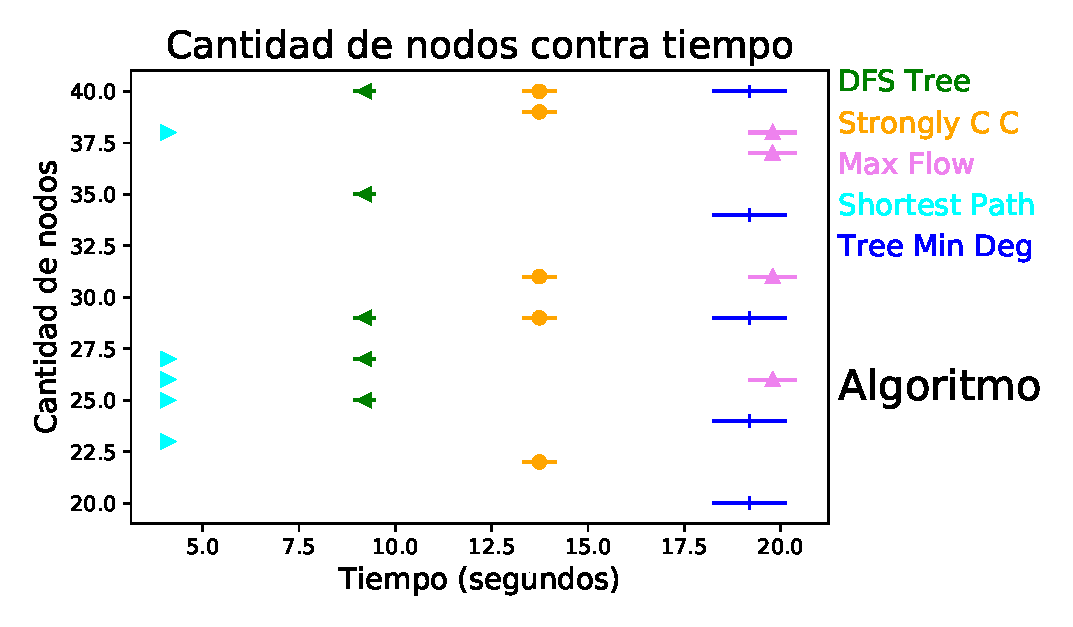
\includegraphics [width=130mm] {scater1.eps}
\caption{Los colores representan a los generadores y las figuras representan algoritmos.}
\label{scater1}
\end{figure}

Se hizo una prueba de correlación entre las variables, para ver si las variables se relacionan entre ellas y con el tiempo de ejecución. Lo que muestra la figura \ref{correlacion} es que el orden y la densidad se relaciona directamente proporcional con el tiempo de ejecución.

\begin{figure}
\centering
\includegraphics [width=100mm] {Correlaciones1.eps}
\caption{Correlaciones entre los datos cuantitativos.}
\label{correlacion}
\end{figure}

Luego, se hizo un ANOVA para identificar si las medias de los conjuntos eran iguales o hay diferencias significativas en ellas. Se obtuvo los resultados que se muestra en la tabla llamada \texttt{ANOVA.txt} en el cual los valores de la tercer columna que son mayores a 0.1, sus medias son iguales y los valores menores 0.1 se rechaza la hipótesis de que las medias sean iguales.

% redefine \VerbatimInput
\RecustomVerbatimCommand{\VerbatimInput}{VerbatimInput}%
{fontsize=\footnotesize,
 %
 frame=lines,  % top and bottom rule only
 framesep=2em, % separation between frame and text
 rulecolor=\color{Gray},
 %
 label=\fbox{\color{Black}ANOVA.txt},
 labelposition=topline,
 %
 commandchars=\|\(\), % escape character and argument delimiters for
                      % commands within the verbatim
 commentchar=*        % comment character
}

\VerbatimInput{Anova1.txt}




\bibliographystyle{IEEEtran}
\bibliography{Bibliog}
\nocite{*}
\end{document}
